\section{Operations}\label{sec:ops}

We define the following operations. Each takes a layout $L$, except
$\mathrm{canonical}$, which takes a shape, and where a second argument is
needed it is written out; $S$ ranges over shapes and $A$ over
layouts.

\begin{description}
\item[$\mathrm{canonical}(S)$] for a flat shape $S = (n_1,\dots,n_k)$, the
layout
\[
(n_1,\dots,n_k) \;{:}\; \Big(\textstyle\prod_{i>1} n_i,\;
\prod_{i>2} n_i,\; \dots,\; n_k,\; 1\Big).
\]
For an entry that is itself a shape, we take the canonical layout
of that shape, with every stride multiplied by the product of the sizes to its
right.
\par\smallskip
\begin{center}
\begin{minipage}[t]{0.6\linewidth}\centering
$\mathrm{canonical}((3,4)) = (3,4){:}(4,1)$\\[4pt]
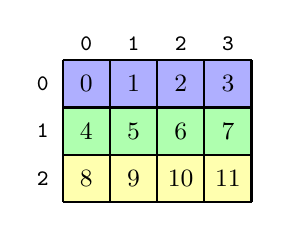
\begin{tikzpicture}[x={(0cm,-0.6cm)},y={(0.6cm,0cm)},every node/.style={minimum size=0.6cm, outer sep=0pt, font=\small}]
\node[fill={rgb,255:red,175;green,175;blue,255}] at (0,0) {0};
\node[fill={rgb,255:red,175;green,175;blue,255}] at (0,1) {1};
\node[fill={rgb,255:red,175;green,175;blue,255}] at (0,2) {2};
\node[fill={rgb,255:red,175;green,175;blue,255}] at (0,3) {3};
\node[fill={rgb,255:red,175;green,255;blue,175}] at (1,0) {4};
\node[fill={rgb,255:red,175;green,255;blue,175}] at (1,1) {5};
\node[fill={rgb,255:red,175;green,255;blue,175}] at (1,2) {6};
\node[fill={rgb,255:red,175;green,255;blue,175}] at (1,3) {7};
\node[fill={rgb,255:red,255;green,255;blue,175}] at (2,0) {8};
\node[fill={rgb,255:red,255;green,255;blue,175}] at (2,1) {9};
\node[fill={rgb,255:red,255;green,255;blue,175}] at (2,2) {10};
\node[fill={rgb,255:red,255;green,255;blue,175}] at (2,3) {11};
\draw[color=black,thick,step=0.6cm,shift={(-0.5,-0.5)}] (0,0) grid (3,4);
\node[anchor=east,minimum size=0pt,font=\footnotesize] at (0,-0.6) {\texttt{0}};
\node[anchor=east,minimum size=0pt,font=\footnotesize] at (1,-0.6) {\texttt{1}};
\node[anchor=east,minimum size=0pt,font=\footnotesize] at (2,-0.6) {\texttt{2}};
\node[minimum size=0pt,font=\footnotesize] at (-0.85,0) {\texttt{0}};
\node[minimum size=0pt,font=\footnotesize] at (-0.85,1) {\texttt{1}};
\node[minimum size=0pt,font=\footnotesize] at (-0.85,2) {\texttt{2}};
\node[minimum size=0pt,font=\footnotesize] at (-0.85,3) {\texttt{3}};
\end{tikzpicture}
\end{minipage}
\end{center}



\item[$\mathrm{split}(n{:}d,\, S)$] for $\size S = n$, the shape $S$ carrying
the strides of $\mathrm{canonical}(S)$ each multiplied by $d$, which for a flat
$S = (m_1,\dots,m_r)$ is
\[
(m_1,\dots,m_r) \;{:}\;
\Big(d\textstyle\prod_{i>1} m_i,\; d\prod_{i>2} m_i,\; \dots,\; d\,m_r,\; d\Big)
\]
and for a nested $S$ follows its nesting. The argument $n{:}\bot$ gives $S$
with every stride $\bot$.
\par\smallskip
\begin{center}
\begin{minipage}[t]{0.5\linewidth}\centering
$6{:}2$\\[4pt]
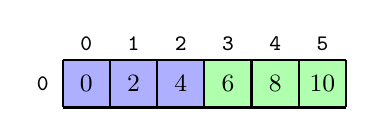
\begin{tikzpicture}[x={(0cm,-0.6cm)},y={(0.6cm,0cm)},every node/.style={minimum size=0.6cm, outer sep=0pt, font=\small}]
\node[fill={rgb,255:red,175;green,175;blue,255}] at (0,0) {0};
\node[fill={rgb,255:red,175;green,175;blue,255}] at (0,1) {2};
\node[fill={rgb,255:red,175;green,175;blue,255}] at (0,2) {4};
\node[fill={rgb,255:red,175;green,255;blue,175}] at (0,3) {6};
\node[fill={rgb,255:red,175;green,255;blue,175}] at (0,4) {8};
\node[fill={rgb,255:red,175;green,255;blue,175}] at (0,5) {10};
\draw[color=black,thick,step=0.6cm,shift={(-0.5,-0.5)}] (0,0) grid (1,6);
\node[anchor=east,minimum size=0pt,font=\footnotesize] at (0,-0.6) {\texttt{0}};
\node[minimum size=0pt,font=\footnotesize] at (-0.85,0) {\texttt{0}};
\node[minimum size=0pt,font=\footnotesize] at (-0.85,1) {\texttt{1}};
\node[minimum size=0pt,font=\footnotesize] at (-0.85,2) {\texttt{2}};
\node[minimum size=0pt,font=\footnotesize] at (-0.85,3) {\texttt{3}};
\node[minimum size=0pt,font=\footnotesize] at (-0.85,4) {\texttt{4}};
\node[minimum size=0pt,font=\footnotesize] at (-0.85,5) {\texttt{5}};
\end{tikzpicture}
\end{minipage}\hfill
\begin{minipage}[t]{0.45\linewidth}\centering
$\mathrm{split}(6{:}2,\,(2,3)) = (2,3){:}(6,2)$\\[4pt]
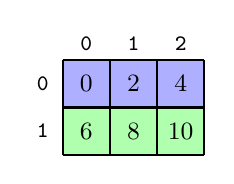
\begin{tikzpicture}[x={(0cm,-0.6cm)},y={(0.6cm,0cm)},every node/.style={minimum size=0.6cm, outer sep=0pt, font=\small}]
\node[fill={rgb,255:red,175;green,175;blue,255}] at (0,0) {0};
\node[fill={rgb,255:red,175;green,175;blue,255}] at (0,1) {2};
\node[fill={rgb,255:red,175;green,175;blue,255}] at (0,2) {4};
\node[fill={rgb,255:red,175;green,255;blue,175}] at (1,0) {6};
\node[fill={rgb,255:red,175;green,255;blue,175}] at (1,1) {8};
\node[fill={rgb,255:red,175;green,255;blue,175}] at (1,2) {10};
\draw[color=black,thick,step=0.6cm,shift={(-0.5,-0.5)}] (0,0) grid (2,3);
\node[anchor=east,minimum size=0pt,font=\footnotesize] at (0,-0.6) {\texttt{0}};
\node[anchor=east,minimum size=0pt,font=\footnotesize] at (1,-0.6) {\texttt{1}};
\node[minimum size=0pt,font=\footnotesize] at (-0.85,0) {\texttt{0}};
\node[minimum size=0pt,font=\footnotesize] at (-0.85,1) {\texttt{1}};
\node[minimum size=0pt,font=\footnotesize] at (-0.85,2) {\texttt{2}};
\end{tikzpicture}
\end{minipage}
\end{center}



\item[$\divideop(L, S)$] partitions $L$ into tiles of shape $S$. Let
$L = (n_1,\dots,n_m){:}(d_1,\dots,d_m)$ and let $S = (k_1,\dots,k_m)$ with
$k_i \mid n_i$. Each mode splits as
\[
\mathrm{split}\big(n_i{:}d_i,\; (n_i/k_i,\, k_i)\big)
\;=\; (n_i/k_i,\, k_i) \;{:}\; (k_i d_i,\, d_i),
\]
and collecting the second component of every split into one group and the
first into another gives
\[
\divideop(L,S) \;=\;
\big((k_1,\dots,k_m),\ (n_1/k_1,\dots,n_m/k_m)\big)
\;{:}\;
\big((d_1,\dots,d_m),\ (k_1d_1,\dots,k_md_m)\big).
\]
The first group indexes a mode inside a tile and the second indexes which
tile. It is easy to see that precomposing with the flattening that sends each pair
$(b_i, t_i)$ back to $c_i = b_i k_i + t_i$ recovers $L$.
\par\smallskip
\begin{center}
\begin{minipage}[t]{0.48\linewidth}\centering
$L = (4,6){:}(6,1)$, coloured by tile\\[4pt]
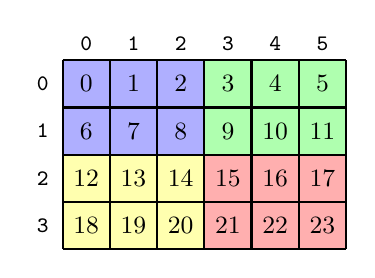
\begin{tikzpicture}[x={(0cm,-0.6cm)},y={(0.6cm,0cm)},every node/.style={minimum size=0.6cm, outer sep=0pt, font=\small}]
\node[fill={rgb,255:red,175;green,175;blue,255}] at (0,0) {0};
\node[fill={rgb,255:red,175;green,175;blue,255}] at (0,1) {1};
\node[fill={rgb,255:red,175;green,175;blue,255}] at (0,2) {2};
\node[fill={rgb,255:red,175;green,255;blue,175}] at (0,3) {3};
\node[fill={rgb,255:red,175;green,255;blue,175}] at (0,4) {4};
\node[fill={rgb,255:red,175;green,255;blue,175}] at (0,5) {5};
\node[fill={rgb,255:red,175;green,175;blue,255}] at (1,0) {6};
\node[fill={rgb,255:red,175;green,175;blue,255}] at (1,1) {7};
\node[fill={rgb,255:red,175;green,175;blue,255}] at (1,2) {8};
\node[fill={rgb,255:red,175;green,255;blue,175}] at (1,3) {9};
\node[fill={rgb,255:red,175;green,255;blue,175}] at (1,4) {10};
\node[fill={rgb,255:red,175;green,255;blue,175}] at (1,5) {11};
\node[fill={rgb,255:red,255;green,255;blue,175}] at (2,0) {12};
\node[fill={rgb,255:red,255;green,255;blue,175}] at (2,1) {13};
\node[fill={rgb,255:red,255;green,255;blue,175}] at (2,2) {14};
\node[fill={rgb,255:red,255;green,175;blue,175}] at (2,3) {15};
\node[fill={rgb,255:red,255;green,175;blue,175}] at (2,4) {16};
\node[fill={rgb,255:red,255;green,175;blue,175}] at (2,5) {17};
\node[fill={rgb,255:red,255;green,255;blue,175}] at (3,0) {18};
\node[fill={rgb,255:red,255;green,255;blue,175}] at (3,1) {19};
\node[fill={rgb,255:red,255;green,255;blue,175}] at (3,2) {20};
\node[fill={rgb,255:red,255;green,175;blue,175}] at (3,3) {21};
\node[fill={rgb,255:red,255;green,175;blue,175}] at (3,4) {22};
\node[fill={rgb,255:red,255;green,175;blue,175}] at (3,5) {23};
\draw[color=black,thick,step=0.6cm,shift={(-0.5,-0.5)}] (0,0) grid (4,6);
\node[anchor=east,minimum size=0pt,font=\footnotesize] at (0,-0.6) {\texttt{0}};
\node[anchor=east,minimum size=0pt,font=\footnotesize] at (1,-0.6) {\texttt{1}};
\node[anchor=east,minimum size=0pt,font=\footnotesize] at (2,-0.6) {\texttt{2}};
\node[anchor=east,minimum size=0pt,font=\footnotesize] at (3,-0.6) {\texttt{3}};
\node[minimum size=0pt,font=\footnotesize] at (-0.85,0) {\texttt{0}};
\node[minimum size=0pt,font=\footnotesize] at (-0.85,1) {\texttt{1}};
\node[minimum size=0pt,font=\footnotesize] at (-0.85,2) {\texttt{2}};
\node[minimum size=0pt,font=\footnotesize] at (-0.85,3) {\texttt{3}};
\node[minimum size=0pt,font=\footnotesize] at (-0.85,4) {\texttt{4}};
\node[minimum size=0pt,font=\footnotesize] at (-0.85,5) {\texttt{5}};
\end{tikzpicture}
\end{minipage}\hfill
\begin{minipage}[t]{0.48\linewidth}\centering
$\divideop(L,(2,3))$: tile coordinate $(t_1,t_2)$ as row, tile $(b_1,b_2)$ as column\\[4pt]
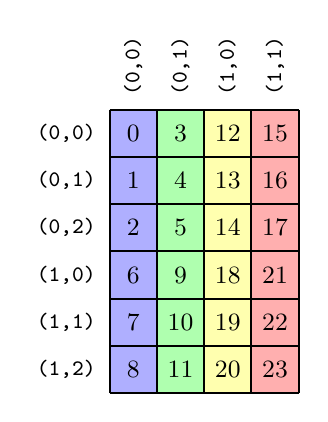
\begin{tikzpicture}[x={(0cm,-0.6cm)},y={(0.6cm,0cm)},every node/.style={minimum size=0.6cm, outer sep=0pt, font=\small}]
\node[fill={rgb,255:red,175;green,175;blue,255}] at (0,0) {0};
\node[fill={rgb,255:red,175;green,255;blue,175}] at (0,1) {3};
\node[fill={rgb,255:red,255;green,255;blue,175}] at (0,2) {12};
\node[fill={rgb,255:red,255;green,175;blue,175}] at (0,3) {15};
\node[fill={rgb,255:red,175;green,175;blue,255}] at (1,0) {1};
\node[fill={rgb,255:red,175;green,255;blue,175}] at (1,1) {4};
\node[fill={rgb,255:red,255;green,255;blue,175}] at (1,2) {13};
\node[fill={rgb,255:red,255;green,175;blue,175}] at (1,3) {16};
\node[fill={rgb,255:red,175;green,175;blue,255}] at (2,0) {2};
\node[fill={rgb,255:red,175;green,255;blue,175}] at (2,1) {5};
\node[fill={rgb,255:red,255;green,255;blue,175}] at (2,2) {14};
\node[fill={rgb,255:red,255;green,175;blue,175}] at (2,3) {17};
\node[fill={rgb,255:red,175;green,175;blue,255}] at (3,0) {6};
\node[fill={rgb,255:red,175;green,255;blue,175}] at (3,1) {9};
\node[fill={rgb,255:red,255;green,255;blue,175}] at (3,2) {18};
\node[fill={rgb,255:red,255;green,175;blue,175}] at (3,3) {21};
\node[fill={rgb,255:red,175;green,175;blue,255}] at (4,0) {7};
\node[fill={rgb,255:red,175;green,255;blue,175}] at (4,1) {10};
\node[fill={rgb,255:red,255;green,255;blue,175}] at (4,2) {19};
\node[fill={rgb,255:red,255;green,175;blue,175}] at (4,3) {22};
\node[fill={rgb,255:red,175;green,175;blue,255}] at (5,0) {8};
\node[fill={rgb,255:red,175;green,255;blue,175}] at (5,1) {11};
\node[fill={rgb,255:red,255;green,255;blue,175}] at (5,2) {20};
\node[fill={rgb,255:red,255;green,175;blue,175}] at (5,3) {23};
\draw[color=black,thick,step=0.6cm,shift={(-0.5,-0.5)}] (0,0) grid (6,4);
\node[anchor=east,minimum size=0pt,font=\footnotesize] at (0,-0.6) {\texttt{(0,0)}};
\node[anchor=east,minimum size=0pt,font=\footnotesize] at (1,-0.6) {\texttt{(0,1)}};
\node[anchor=east,minimum size=0pt,font=\footnotesize] at (2,-0.6) {\texttt{(0,2)}};
\node[anchor=east,minimum size=0pt,font=\footnotesize] at (3,-0.6) {\texttt{(1,0)}};
\node[anchor=east,minimum size=0pt,font=\footnotesize] at (4,-0.6) {\texttt{(1,1)}};
\node[anchor=east,minimum size=0pt,font=\footnotesize] at (5,-0.6) {\texttt{(1,2)}};
\node[rotate=90,anchor=west,minimum size=0pt,font=\footnotesize] at (-0.6,0) {\texttt{(0,0)}};
\node[rotate=90,anchor=west,minimum size=0pt,font=\footnotesize] at (-0.6,1) {\texttt{(0,1)}};
\node[rotate=90,anchor=west,minimum size=0pt,font=\footnotesize] at (-0.6,2) {\texttt{(1,0)}};
\node[rotate=90,anchor=west,minimum size=0pt,font=\footnotesize] at (-0.6,3) {\texttt{(1,1)}};
\end{tikzpicture}
\end{minipage}
\end{center}



\item[$\repeatop(L, A)$] copies of $L$ arranged in the layout of $A$, which is
required to be a valid $\logical \to \logical$ layout and so a dense bijection:
\[
\repeatop(L,A) \;=\; (S_A, S_L) \;{:}\; \big((\cosize L)\,D_A,\ D_L\big),
\]
where $L = S_L{:}D_L$, $A = S_A{:}D_A$, and $c\,D$ multiplies every stride of
$D$ by $c$.
If $L$ is a dense bijection then $\cosize L = \size L$, and the addresses
$(\size L)\,A(a) + L(v)$ take every value in $[0, \size A \cdot \size L)$
exactly once: the result is a dense bijection.

When $L$ carries a swizzle $\sigma$, $\repeatop$ is defined only if $\cosize L$
is a power of two, $2^p$, and both fields of $\sigma$ lie below bit $p$. Then
$\sigma\big((\cosize L)\,a + x\big) = (\cosize L)\,a + \sigma(x)$ and every
copy is swizzled alike. Otherwise the copy index reaches the bits $\sigma$
reads, and the operation rejects.

\item[$\interleave(L, A)$] the same copies interleaved element by element
rather than laid out one after another, with $A$ again a valid
$\logical \to \logical$ layout:
\[
\interleave(L,A) \;=\; (S_A, S_L) \;{:}\; \big(D_A,\ (\size A)\,D_L\big).
\]
The coordinate $(a,v)$ lands at $A(a) + (\size A)\,L(v)$, so each element of
$L$ becomes a run of $\size A$ consecutive addresses holding that element of
every copy, where $\repeatop$ instead gives each copy a run of its own. If $L$
is a dense bijection the result is again a dense bijection onto
$[0, \size A \cdot \size L)$. On a swizzled $L$ it has no defined meaning
and rejects.
\par\smallskip
\begin{center}
\begin{minipage}[t]{0.2\linewidth}\centering
$L = (2,2){:}(2,1)$\\[4pt]
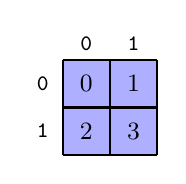
\begin{tikzpicture}[x={(0cm,-0.6cm)},y={(0.6cm,0cm)},every node/.style={minimum size=0.6cm, outer sep=0pt, font=\small}]
\node[fill={rgb,255:red,175;green,175;blue,255}] at (0,0) {0};
\node[fill={rgb,255:red,175;green,175;blue,255}] at (0,1) {1};
\node[fill={rgb,255:red,175;green,175;blue,255}] at (1,0) {2};
\node[fill={rgb,255:red,175;green,175;blue,255}] at (1,1) {3};
\draw[color=black,thick,step=0.6cm,shift={(-0.5,-0.5)}] (0,0) grid (2,2);
\node[anchor=east,minimum size=0pt,font=\footnotesize] at (0,-0.6) {\texttt{0}};
\node[anchor=east,minimum size=0pt,font=\footnotesize] at (1,-0.6) {\texttt{1}};
\node[minimum size=0pt,font=\footnotesize] at (-0.85,0) {\texttt{0}};
\node[minimum size=0pt,font=\footnotesize] at (-0.85,1) {\texttt{1}};
\end{tikzpicture}
\end{minipage}\hfill
\begin{minipage}[t]{0.38\linewidth}\centering
$\repeatop(L,\,3{:}1) = (3,(2,2)){:}(4,(2,1))$\\[4pt]
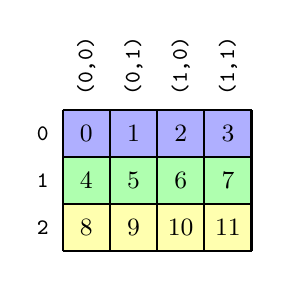
\begin{tikzpicture}[x={(0cm,-0.6cm)},y={(0.6cm,0cm)},every node/.style={minimum size=0.6cm, outer sep=0pt, font=\small}]
\node[fill={rgb,255:red,175;green,175;blue,255}] at (0,0) {0};
\node[fill={rgb,255:red,175;green,175;blue,255}] at (0,1) {1};
\node[fill={rgb,255:red,175;green,175;blue,255}] at (0,2) {2};
\node[fill={rgb,255:red,175;green,175;blue,255}] at (0,3) {3};
\node[fill={rgb,255:red,175;green,255;blue,175}] at (1,0) {4};
\node[fill={rgb,255:red,175;green,255;blue,175}] at (1,1) {5};
\node[fill={rgb,255:red,175;green,255;blue,175}] at (1,2) {6};
\node[fill={rgb,255:red,175;green,255;blue,175}] at (1,3) {7};
\node[fill={rgb,255:red,255;green,255;blue,175}] at (2,0) {8};
\node[fill={rgb,255:red,255;green,255;blue,175}] at (2,1) {9};
\node[fill={rgb,255:red,255;green,255;blue,175}] at (2,2) {10};
\node[fill={rgb,255:red,255;green,255;blue,175}] at (2,3) {11};
\draw[color=black,thick,step=0.6cm,shift={(-0.5,-0.5)}] (0,0) grid (3,4);
\node[anchor=east,minimum size=0pt,font=\footnotesize] at (0,-0.6) {\texttt{0}};
\node[anchor=east,minimum size=0pt,font=\footnotesize] at (1,-0.6) {\texttt{1}};
\node[anchor=east,minimum size=0pt,font=\footnotesize] at (2,-0.6) {\texttt{2}};
\node[rotate=90,anchor=west,minimum size=0pt,font=\footnotesize] at (-0.6,0) {\texttt{(0,0)}};
\node[rotate=90,anchor=west,minimum size=0pt,font=\footnotesize] at (-0.6,1) {\texttt{(0,1)}};
\node[rotate=90,anchor=west,minimum size=0pt,font=\footnotesize] at (-0.6,2) {\texttt{(1,0)}};
\node[rotate=90,anchor=west,minimum size=0pt,font=\footnotesize] at (-0.6,3) {\texttt{(1,1)}};
\end{tikzpicture}
\end{minipage}\hfill
\begin{minipage}[t]{0.38\linewidth}\centering
$\interleave(L,\,3{:}1) = (3,(2,2)){:}(1,(6,3))$\\[4pt]
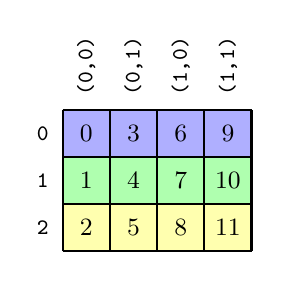
\begin{tikzpicture}[x={(0cm,-0.6cm)},y={(0.6cm,0cm)},every node/.style={minimum size=0.6cm, outer sep=0pt, font=\small}]
\node[fill={rgb,255:red,175;green,175;blue,255}] at (0,0) {0};
\node[fill={rgb,255:red,175;green,175;blue,255}] at (0,1) {3};
\node[fill={rgb,255:red,175;green,175;blue,255}] at (0,2) {6};
\node[fill={rgb,255:red,175;green,175;blue,255}] at (0,3) {9};
\node[fill={rgb,255:red,175;green,255;blue,175}] at (1,0) {1};
\node[fill={rgb,255:red,175;green,255;blue,175}] at (1,1) {4};
\node[fill={rgb,255:red,175;green,255;blue,175}] at (1,2) {7};
\node[fill={rgb,255:red,175;green,255;blue,175}] at (1,3) {10};
\node[fill={rgb,255:red,255;green,255;blue,175}] at (2,0) {2};
\node[fill={rgb,255:red,255;green,255;blue,175}] at (2,1) {5};
\node[fill={rgb,255:red,255;green,255;blue,175}] at (2,2) {8};
\node[fill={rgb,255:red,255;green,255;blue,175}] at (2,3) {11};
\draw[color=black,thick,step=0.6cm,shift={(-0.5,-0.5)}] (0,0) grid (3,4);
\node[anchor=east,minimum size=0pt,font=\footnotesize] at (0,-0.6) {\texttt{0}};
\node[anchor=east,minimum size=0pt,font=\footnotesize] at (1,-0.6) {\texttt{1}};
\node[anchor=east,minimum size=0pt,font=\footnotesize] at (2,-0.6) {\texttt{2}};
\node[rotate=90,anchor=west,minimum size=0pt,font=\footnotesize] at (-0.6,0) {\texttt{(0,0)}};
\node[rotate=90,anchor=west,minimum size=0pt,font=\footnotesize] at (-0.6,1) {\texttt{(0,1)}};
\node[rotate=90,anchor=west,minimum size=0pt,font=\footnotesize] at (-0.6,2) {\texttt{(1,0)}};
\node[rotate=90,anchor=west,minimum size=0pt,font=\footnotesize] at (-0.6,3) {\texttt{(1,1)}};
\end{tikzpicture}
\end{minipage}
\end{center}



\item[$\broadcast(L, S)$] $\size S$ copies of $L$ at the same addresses:
\[
\broadcast(L,S) \;=\; (S, S_L) \;{:}\; (\bot,\ D_L),
\]
writing $\bot$ for the stride with $\bot$ at every entry of $S$. The coordinate
$(a,v)$ lands at $L(v)$ whatever $a$ is. The second argument is a shape and not
a layout because the copies share their addresses and so have no strides to
carry. The result is valid when $L$ is, and not write-valid once
$\size S \ge 2$.
\par\smallskip
\begin{center}
\begin{minipage}[t]{0.6\linewidth}\centering
$\broadcast(4{:}1,\,(3)) = (3,4){:}(\bot,1)$: copy as row\\[4pt]
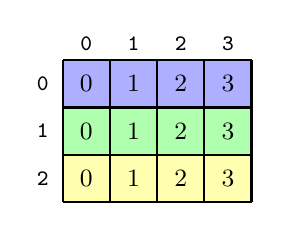
\begin{tikzpicture}[x={(0cm,-0.6cm)},y={(0.6cm,0cm)},every node/.style={minimum size=0.6cm, outer sep=0pt, font=\small}]
\node[fill={rgb,255:red,175;green,175;blue,255}] at (0,0) {0};
\node[fill={rgb,255:red,175;green,175;blue,255}] at (0,1) {1};
\node[fill={rgb,255:red,175;green,175;blue,255}] at (0,2) {2};
\node[fill={rgb,255:red,175;green,175;blue,255}] at (0,3) {3};
\node[fill={rgb,255:red,175;green,255;blue,175}] at (1,0) {0};
\node[fill={rgb,255:red,175;green,255;blue,175}] at (1,1) {1};
\node[fill={rgb,255:red,175;green,255;blue,175}] at (1,2) {2};
\node[fill={rgb,255:red,175;green,255;blue,175}] at (1,3) {3};
\node[fill={rgb,255:red,255;green,255;blue,175}] at (2,0) {0};
\node[fill={rgb,255:red,255;green,255;blue,175}] at (2,1) {1};
\node[fill={rgb,255:red,255;green,255;blue,175}] at (2,2) {2};
\node[fill={rgb,255:red,255;green,255;blue,175}] at (2,3) {3};
\draw[color=black,thick,step=0.6cm,shift={(-0.5,-0.5)}] (0,0) grid (3,4);
\node[anchor=east,minimum size=0pt,font=\footnotesize] at (0,-0.6) {\texttt{0}};
\node[anchor=east,minimum size=0pt,font=\footnotesize] at (1,-0.6) {\texttt{1}};
\node[anchor=east,minimum size=0pt,font=\footnotesize] at (2,-0.6) {\texttt{2}};
\node[minimum size=0pt,font=\footnotesize] at (-0.85,0) {\texttt{0}};
\node[minimum size=0pt,font=\footnotesize] at (-0.85,1) {\texttt{1}};
\node[minimum size=0pt,font=\footnotesize] at (-0.85,2) {\texttt{2}};
\node[minimum size=0pt,font=\footnotesize] at (-0.85,3) {\texttt{3}};
\end{tikzpicture}
\end{minipage}
\end{center}



\item[$\mathrm{inverse}(L)$] for $L$ a flat dense bijection with modes
$(n_1,\dots,n_m){:}(d_1,\dots,d_m)$, every $n_i \ge 2$; as in
Lemma~\ref{lem:dense}, modes of size $1$ are dropped first. Give mode $i$ the canonical weight
$w_i = \prod_{j>i} n_j$ and list the modes in decreasing order of stride. Then
\[
\mathrm{inverse}(L) \;=\;
(n_{(1)},\dots,n_{(m)}) \;{:}\; (w_{(1)},\dots,w_{(m)}),
\]
again a dense bijection. Read both as maps on $[0,N)$, each unflattening the
integer it is given into its own shape, and they are mutually inverse.
\par\smallskip
\begin{center}
\begin{minipage}[t]{0.45\linewidth}\centering
$L = (2,3){:}(1,2)$, coloured by element\\[4pt]
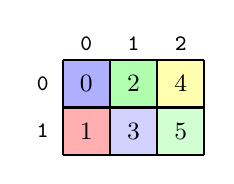
\begin{tikzpicture}[x={(0cm,-0.6cm)},y={(0.6cm,0cm)},every node/.style={minimum size=0.6cm, outer sep=0pt, font=\small}]
\node[fill={rgb,255:red,175;green,175;blue,255}] at (0,0) {0};
\node[fill={rgb,255:red,175;green,255;blue,175}] at (0,1) {2};
\node[fill={rgb,255:red,255;green,255;blue,175}] at (0,2) {4};
\node[fill={rgb,255:red,255;green,175;blue,175}] at (1,0) {1};
\node[fill={rgb,255:red,210;green,210;blue,255}] at (1,1) {3};
\node[fill={rgb,255:red,210;green,255;blue,210}] at (1,2) {5};
\draw[color=black,thick,step=0.6cm,shift={(-0.5,-0.5)}] (0,0) grid (2,3);
\node[anchor=east,minimum size=0pt,font=\footnotesize] at (0,-0.6) {\texttt{0}};
\node[anchor=east,minimum size=0pt,font=\footnotesize] at (1,-0.6) {\texttt{1}};
\node[minimum size=0pt,font=\footnotesize] at (-0.85,0) {\texttt{0}};
\node[minimum size=0pt,font=\footnotesize] at (-0.85,1) {\texttt{1}};
\node[minimum size=0pt,font=\footnotesize] at (-0.85,2) {\texttt{2}};
\end{tikzpicture}
\end{minipage}\hfill
\begin{minipage}[t]{0.5\linewidth}\centering
$\mathrm{inverse}(L) = (3,2){:}(1,3)$, at address $2a+b$ the element $a+3b$\\[4pt]
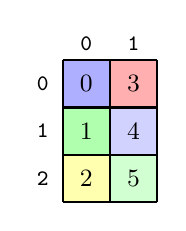
\begin{tikzpicture}[x={(0cm,-0.6cm)},y={(0.6cm,0cm)},every node/.style={minimum size=0.6cm, outer sep=0pt, font=\small}]
\node[fill={rgb,255:red,175;green,175;blue,255}] at (0,0) {0};
\node[fill={rgb,255:red,255;green,175;blue,175}] at (0,1) {3};
\node[fill={rgb,255:red,175;green,255;blue,175}] at (1,0) {1};
\node[fill={rgb,255:red,210;green,210;blue,255}] at (1,1) {4};
\node[fill={rgb,255:red,255;green,255;blue,175}] at (2,0) {2};
\node[fill={rgb,255:red,210;green,255;blue,210}] at (2,1) {5};
\draw[color=black,thick,step=0.6cm,shift={(-0.5,-0.5)}] (0,0) grid (3,2);
\node[anchor=east,minimum size=0pt,font=\footnotesize] at (0,-0.6) {\texttt{0}};
\node[anchor=east,minimum size=0pt,font=\footnotesize] at (1,-0.6) {\texttt{1}};
\node[anchor=east,minimum size=0pt,font=\footnotesize] at (2,-0.6) {\texttt{2}};
\node[minimum size=0pt,font=\footnotesize] at (-0.85,0) {\texttt{0}};
\node[minimum size=0pt,font=\footnotesize] at (-0.85,1) {\texttt{1}};
\end{tikzpicture}
\end{minipage}
\end{center}


\end{description}
